%% Supplementary Data for
%% ChimeraLM: a language model enables accurate structural variant detection
%% in whole-genome amplified long-read sequencing
%%
%% Compiled separately from the main manuscript (sn-article.tex).
%% Build: latexmk -pdf supplementary.tex
%% No revision marks are used in this file (journal requirement).

\documentclass[pdflatex]{sn-jnl}% no sn-* reference option: the NAR style is loaded below

\usepackage{graphicx}%
\usepackage{multirow}%
\usepackage{amsmath,amssymb,amsfonts}%
\usepackage{amsthm}%
\usepackage{mathrsfs}%
\usepackage{xcolor}%
\usepackage{textcomp}%
\usepackage{manyfoot}%
\usepackage{booktabs}%
\usepackage{geometry}

% Journal reference style (Nucleic Acids Research), as in sn-article.tex.
\usepackage[numbers,sort&compress]{natbib}
\gdef\NumBib{YES}
\bibliographystyle{nar}
\setlength{\bibsep}{1em}
\makeatletter
\def\bibfont{\reset@font\fontfamily{\rmdefault}\normalsize\selectfont}
\makeatother

\graphicspath{{../figures}}

\usepackage[acronym, automake, style=index, shortcuts]{glossaries-extra}
\setabbreviationstyle[acronym]{long-short}
\makeglossaries

\newacronym{wga}{WGA}{whole genome amplification}
\newacronym{wgs}{WGS}{whole genome sequencing}
\newacronym{mda}{MDA}{multiple displacement amplification}
\newacronym{malbac}{MALBAC}{multiple annealing and looping-based amplification cycles}
\newacronym{gpu}{GPU}{graphics processing unit}
\newacronym{cpu}{CPU}{central processing unit}
\newacronym{hpc}{HPC}{high performance computing}
\newacronym{sv}{SV}{structural variation}
\newacronym{snp}{SNP}{single nucleotide polymorphism}
\newacronym{ont}{ONT}{Oxford Nanopore Technologies}
\newacronym{pb}{PacBio}{Pacific Biosciences}
\newacronym{del}{DEL}{deletion}
\newacronym{dup}{DUP}{duplication}
\newacronym{ins}{INS}{insertion}
\newacronym{inv}{INV}{inversion}
\newacronym{tra}{TRA}{translocation}
\newacronym{pcr}{PCR}{polymerase chain reaction}
\newacronym{mrna}{mRNA}{messenger RNA}
\newacronym{facs}{FACS}{fluorescence-activated cell sorting}
\newacronym{sa}{SA}{supplementary alignment}
\newacronym{lianti}{LIANTI}{linear amplification via transposon insertion}
\newacronym{doppcr}{DOP-PCR}{degenerate oligonucleotide-primed PCR}
\newacronym{pta}{PTA}{primary template-directed amplification}
\newacronym{dmda}{dMDA}{droplet-based MDA}
\newacronym{ide}{IDE}{integrated development environment}
\newacronym{cd}{CD}{continuous development}
\newacronym{ucsc}{UCSC}{UCSC Genome Browser}
\newacronym{glm}{GLM}{genomic language model}
\newacronym{lcglm}{LCGLM}{long-context genomic language model}
\newacronym{mlp}{MLP}{multilayer perceptron}
\newacronym{gelu}{GELU}{Gaussian error linear unit}

\raggedbottom

% Supplementary numbering: Supplementary Figure S1, Supplementary Table S1
\renewcommand{\figurename}{Supplementary Figure}
\renewcommand{\tablename}{Supplementary Table}
\renewcommand{\thefigure}{S\arabic{figure}}
\renewcommand{\thetable}{S\arabic{table}}

\begin{document}

\title[Supplementary Data]{Supplementary Data for\\ChimeraLM: a language model enables accurate structural variant detection in whole-genome amplified long-read sequencing}

\author[1]{\fnm{Yangyang} \sur{Li}}\email{yangyang.li@northwestern.edu}
\equalcont{These authors contributed equally to this work.}
\author[1]{\fnm{Qingxiang} \sur{Guo}}\email{qingxiang.guo@northwestern.edu}
\equalcont{These authors contributed equally to this work.}
\author*[1,2]{\fnm{Rendong} \sur{Yang}}\email{rendong.yang@northwestern.edu}

\affil[1]{\orgdiv{Department of Urology}, \orgname{Northwestern University Feinberg School of Medicine}, \orgaddress{\street{303 E Superior St}, \city{Chicago}, \postcode{60611}, \state{IL}, \country{USA}}}
\affil[2]{\orgdiv{Robert H. Lurie Comprehensive Cancer Center}, \orgname{Northwestern University Feinberg School of Medicine}, \orgaddress{\street{675 N St Clair St}, \city{Chicago}, \postcode{60611}, \state{IL}, \country{USA}}}

\maketitle

\glsresetall

\section*{Contents}
\begin{itemize}
	\item Supplementary Table S1. Sequencing and alignment statistics of PC3
	\item Supplementary Figure S1. Training dataset construction and bulk-supported labeling strategy
	\item Supplementary Figure S2. Read-length distribution of chimeric reads and length dependence of ChimeraLM classification
	\item Supplementary Figure S3. External validation of the trained model on single-cell WGA data of an independent cell line (HCC78)
	\item Supplementary Figure S4. Overlap of structural variant calls among the four bulk PC3 datasets used to build the gold standard
	\item Supplementary Figure S5. Features of structural variant calls that remain unsupported after ChimeraLM filtering
	\item Supplementary Figure S6. Concordance of structural variant calls among the three bulk PC3 long-read datasets
	\item Supplementary Figure S7. Composition of artifact-supported SVs for PromethION and MinION
	\item Abbreviations
	\item Supplementary References
\end{itemize}

\clearpage

\section*{Supplementary Tables}

\begin{table}[!ht]
	\centering
	\caption{Sequencing and alignment statistics of PC3}
	\label{tab:seq_stats}
	\small
	\setlength{\tabcolsep}{3pt} % Reduce column spacing (default is 6pt)
	\begin{tabular}{@{}llcccccccc@{}}
		\toprule
		\textbf{Sample} & \textbf{Platform} & \textbf{Reads}  & \textbf{Total} & \textbf{Total bases} & \textbf{Fraction} & \textbf{Mean}   & \textbf{Mean}    & \textbf{Average}  \\
		                &                   & ($\times 10^6$) & \textbf{bases} & \textbf{aligned}     & \textbf{aligned}  & \textbf{length} & \textbf{quality} & \textbf{identity} \\
		                &                   &                 & (Gb)           & (Gb)                 &                   & (bp)            & (Q)              & (\%)              \\
		\midrule
		\gls{wga}       & MinION            & 9.11            & 14.6           & 10.4                 & 0.7               & 1,603           & 14.3             & 97.6              \\
		\gls{wga}       & PromethION        & 44.69           & 128.2          & 69.2                 & 0.5               & 2,869           & 14.5             & 96.1              \\
		Bulk            & MinION            & 0.97            & 8.1            & 7.1                  & 0.9               & 8,310           & 17.2             & 97.3              \\
		Bulk            & PromethION        & 8.00            & 69.9           & 62.4                 & 0.9               & 8,732           & 18.5             & 97.7              \\
		\bottomrule
	\end{tabular}
\end{table}

\clearpage

\section*{Supplementary Figures}

\begin{figure}[!ht]
	\begin{center}
		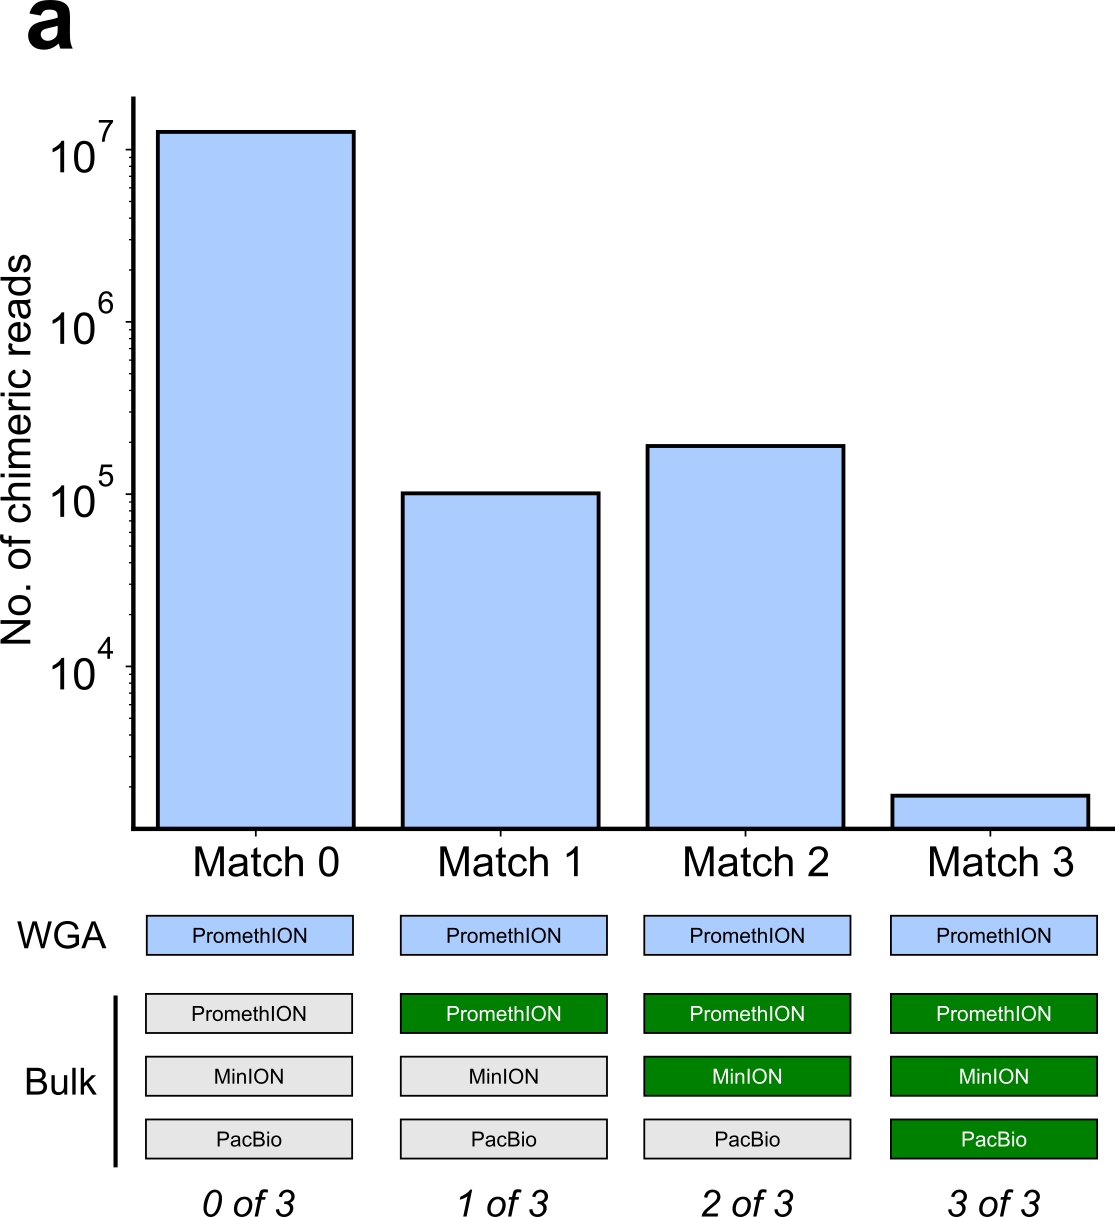
\includegraphics[width=0.9\textwidth]{final_figures/sf1}
	\end{center}
	\caption{{\bf Training dataset construction and bulk-supported labeling strategy.}
		\textbf{(a)}~Workflow for generating labeled training data.
		\gls{wga} PromethION data is compared against three independent bulk sequencing datasets (PromethION, MinION, and PacBio).
		Reads with no bulk matches (Match 0) are labeled artificial; reads matching one or more bulk datasets (Match 1–3) are labeled biological, along with chimeric reads sampled directly from bulk data. The labeled dataset is split into training (70\%), validation (20\%), and test (10\%) sets. The \gls{wga} MinION dataset is reserved for independent cross-platform evaluation.
		\textbf{(b)}~Distribution of chimeric read matches. Bar chart shows the number of \gls{wga} PromethION chimeric reads (log scale) by bulk dataset matches. Match 0 reads (${\sim}10^7$) lacking bulk validation are classified as artificial; Match 1–3 reads with bulk support are classified as biological. The substantial imbalance reflects high prevalence of \gls{wga}-induced artifacts.
	}\label{fig:data_construction}
\end{figure}

\clearpage

\begin{figure}[!ht]
	\begin{center}
		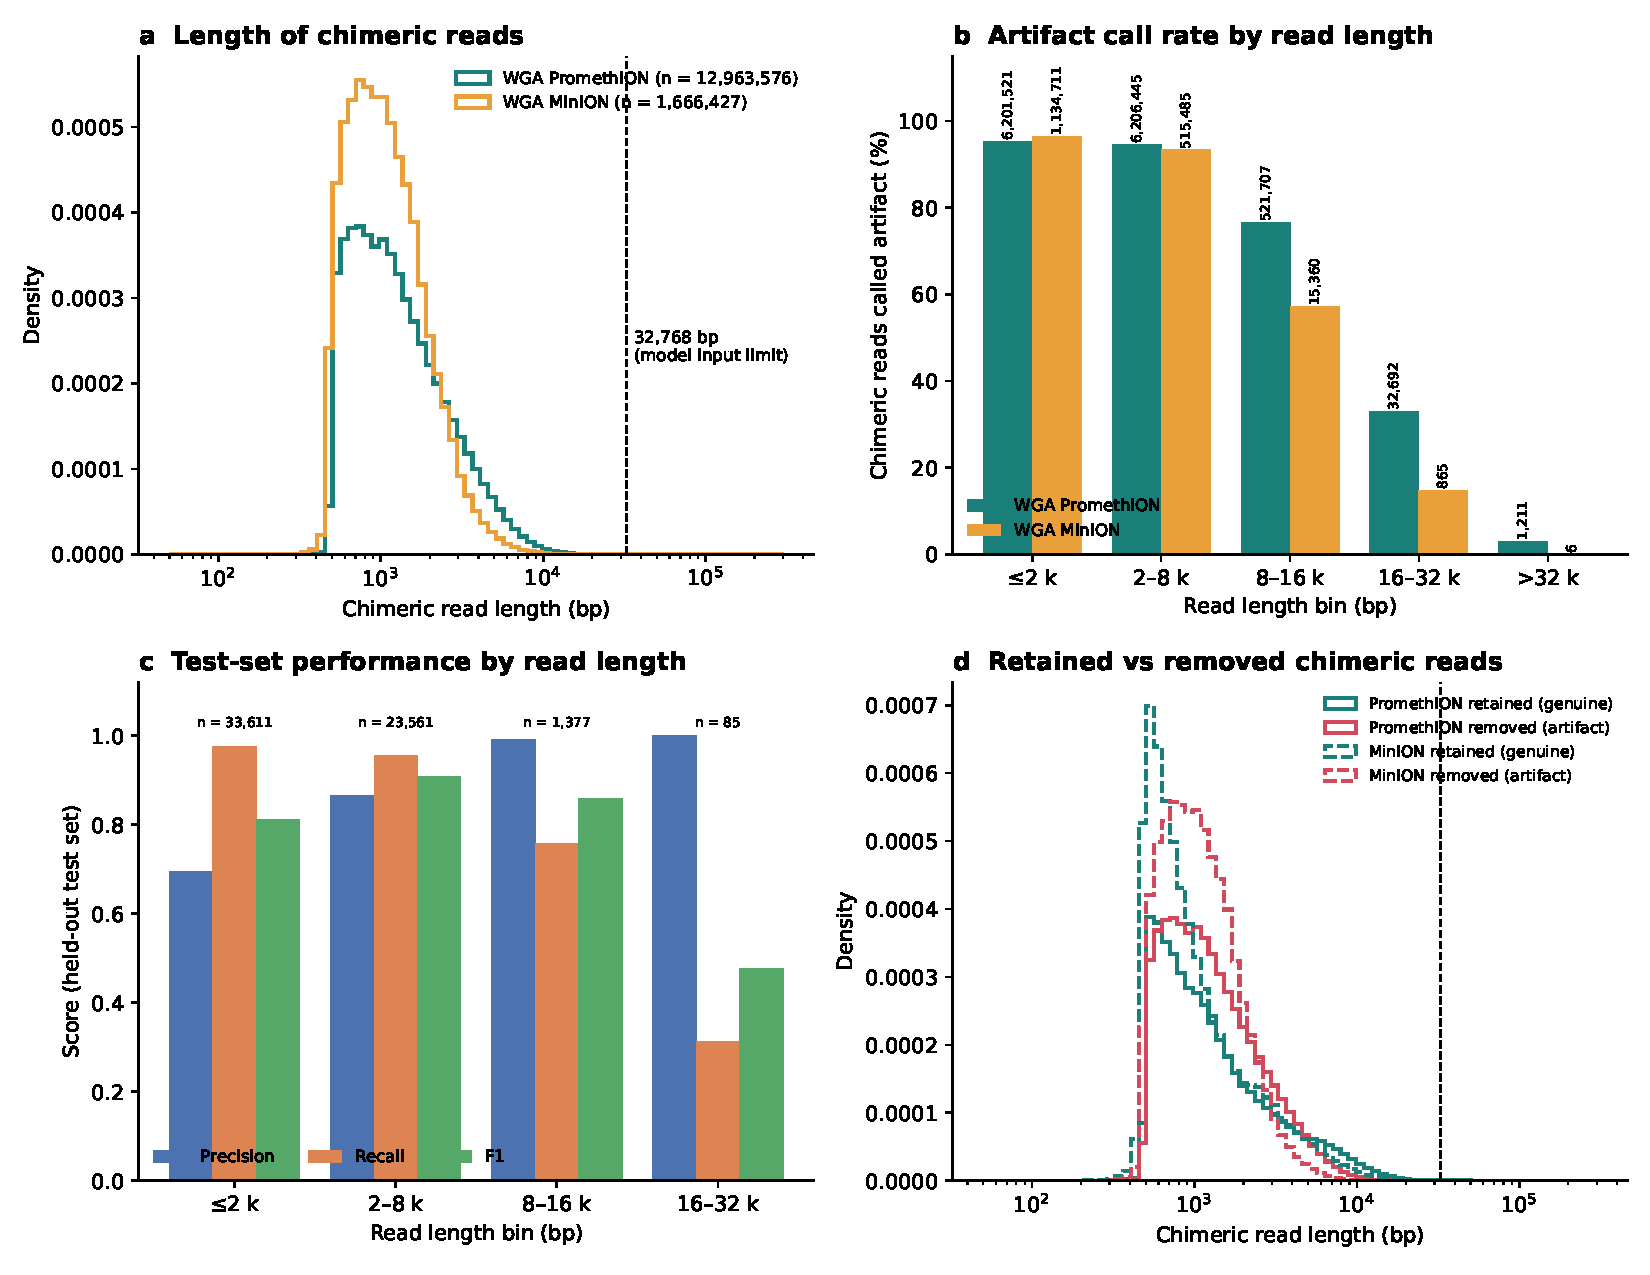
\includegraphics[width=\textwidth]{final_figures/sf_read_length}
	\end{center}
	\caption{{\bf Read-length distribution of chimeric reads and length dependence of ChimeraLM classification.}
		\textbf{(a)}~Length distribution of chimeric reads (primary alignments carrying an \gls{sa} tag) in the \gls{wga} PromethION ($n = 12{,}963{,}576$; median 2,100 bp, N50 4,053 bp, maximum 126,974 bp) and \gls{wga} MinION ($n = 1{,}666{,}427$; median 1,469 bp, N50 2,333 bp, maximum 42,118 bp) datasets. The dashed line marks the 32,768-bp model input limit, exceeded by 1,211 (0.009\%) and 6 reads, respectively; for all but two of these reads at least one chimeric junction lies within the first 32,768 bp.
		\textbf{(b)}~Fraction of chimeric reads classified as \gls{wga}-induced artifacts by read-length bin; numbers above bars give the number of reads per bin.
		\textbf{(c)}~Precision, recall and F1 of ChimeraLM on \gls{wga}-derived held-out test reads ($n = 58{,}636$; the 17,876 test reads sampled from bulk data are not shown because they are not part of the \gls{wga} dataset) stratified by read length. Bins with fewer than 10 reads are omitted.
		\textbf{(d)}~Length distributions of chimeric reads retained (classified as genuine) and removed (classified as artifact) by ChimeraLM on both platforms (PromethION retained: median 3,087 bp, N50 7,989 bp; removed: median 2,067 bp, N50 3,836 bp; MinION retained: median 2,031 bp, N50 5,560 bp; removed: median 1,458 bp, N50 2,220 bp).
	}\label{fig:read_length}
\end{figure}

\clearpage

\begin{figure}[!ht]
	\begin{center}
		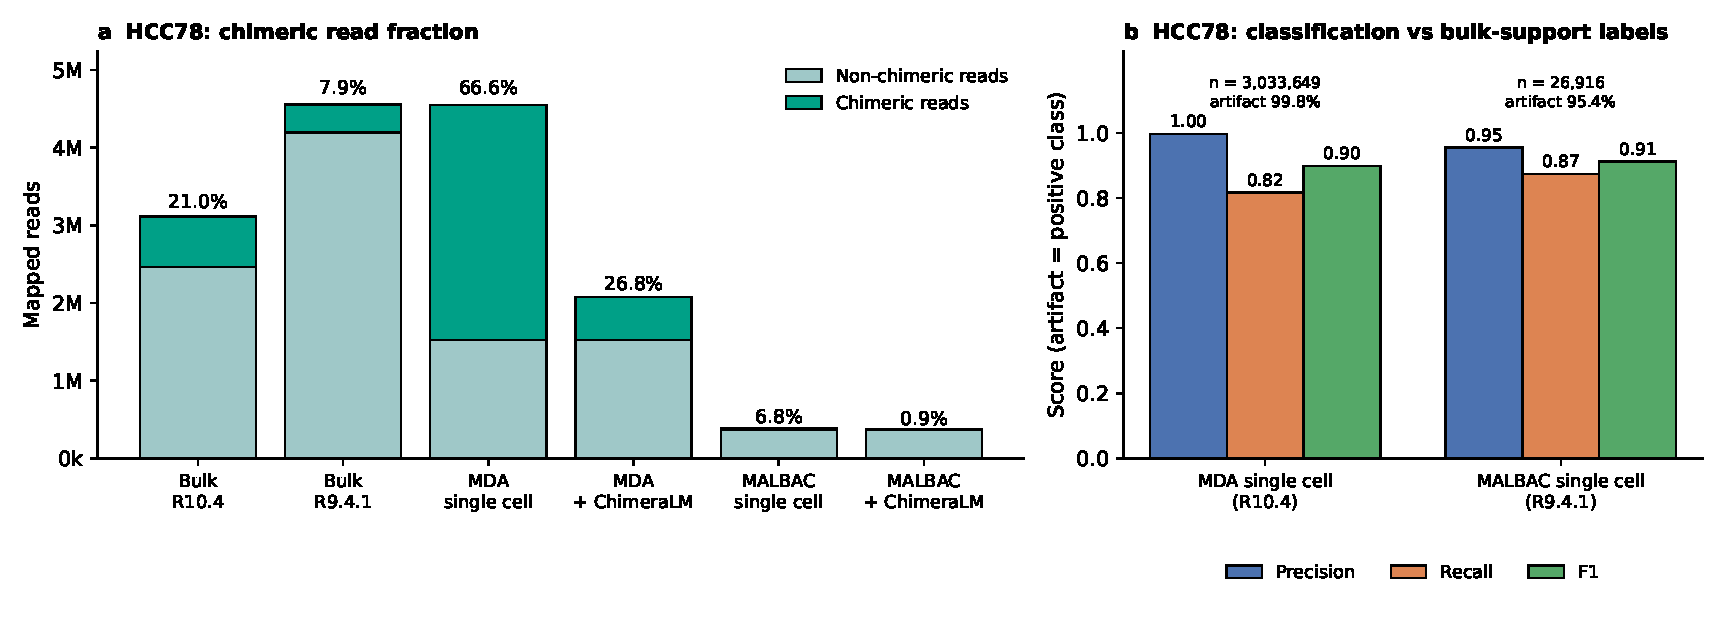
\includegraphics[width=\textwidth]{final_figures/sf_hcc78}
	\end{center}
	\caption{{\bf External validation of the trained model on single-cell WGA data of an independent cell line (HCC78).}
		Data from Ni et al.~\cite{ni2023benchmarking} (NCBI BioProject PRJNA875576): single HCC78 cells amplified with REPLI-g Single Cell \gls{mda} (R10.4 flow cell) or \gls{malbac} (R9.4.1), and two unamplified bulk libraries (R10.4, R9.4.1). The PC3-trained ChimeraLM model was applied without retraining.
		\textbf{(a)}~Chimeric (dark teal) and non-chimeric (light teal) mapped reads with the chimeric fraction above each bar, for the bulk libraries, the \gls{wga} libraries, and the \gls{wga} libraries after ChimeraLM filtering (\gls{mda}: 66.6\% to 26.8\%; \gls{malbac}: 6.8\% to 0.9\%).
		\textbf{(b)}~Precision, recall and F1 for the artifact class against bulk-support labels derived from the two HCC78 bulk libraries (same matching procedure as for PC3); $n$ is the number of labelled chimeric reads and the percentage labelled artifact is given.
	}\label{fig:hcc78}
\end{figure}

\clearpage

\begin{figure}[!ht]
	\begin{center}
		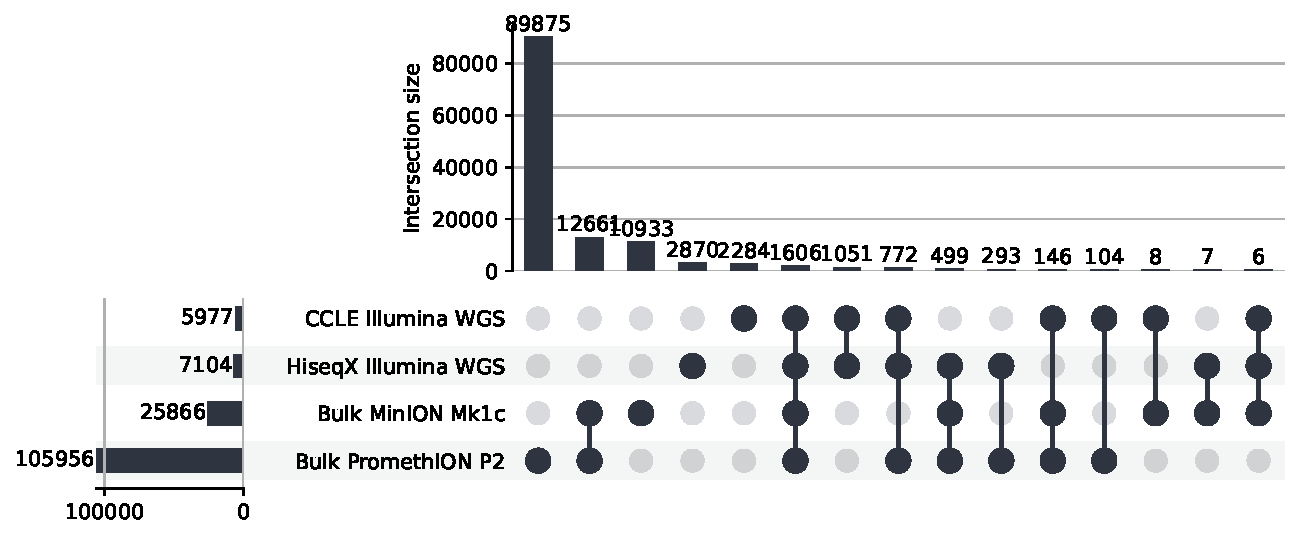
\includegraphics[width=0.95\textwidth]{final_figures/sf_gold_standard_upset}
	\end{center}
	\caption{{\bf Overlap of structural variant calls among the four bulk PC3 datasets used to build the gold standard.}
		UpSet plot of caller-consensus \glspl{sv} ($\geq$2 callers per dataset) from bulk \gls{ont} MinION Mk1c (25,866 calls), bulk \gls{ont} PromethION P2 (105,956), CCLE Illumina \gls{wgs} (5,977) and PRJNA361315 (HiSeq~X) Illumina \gls{wgs} (7,104), merged with OctopuSV. The union contains 123,115 events; 17,153 are supported by $\geq$2 datasets (the gold standard used in Figure~3 of the main text), 3,029 by $\geq$3 and 1,606 by all four. Within the $\geq$2 set, 12,661 events (73.8\%) are shared only by the two long-read datasets, 3,441 (20.1\%) have both long- and short-read support and 1,051 (6.1\%) are shared only by the two short-read datasets.
	}\label{fig:gold_standard}
\end{figure}

\clearpage

\begin{figure}[!ht]
	\begin{center}
		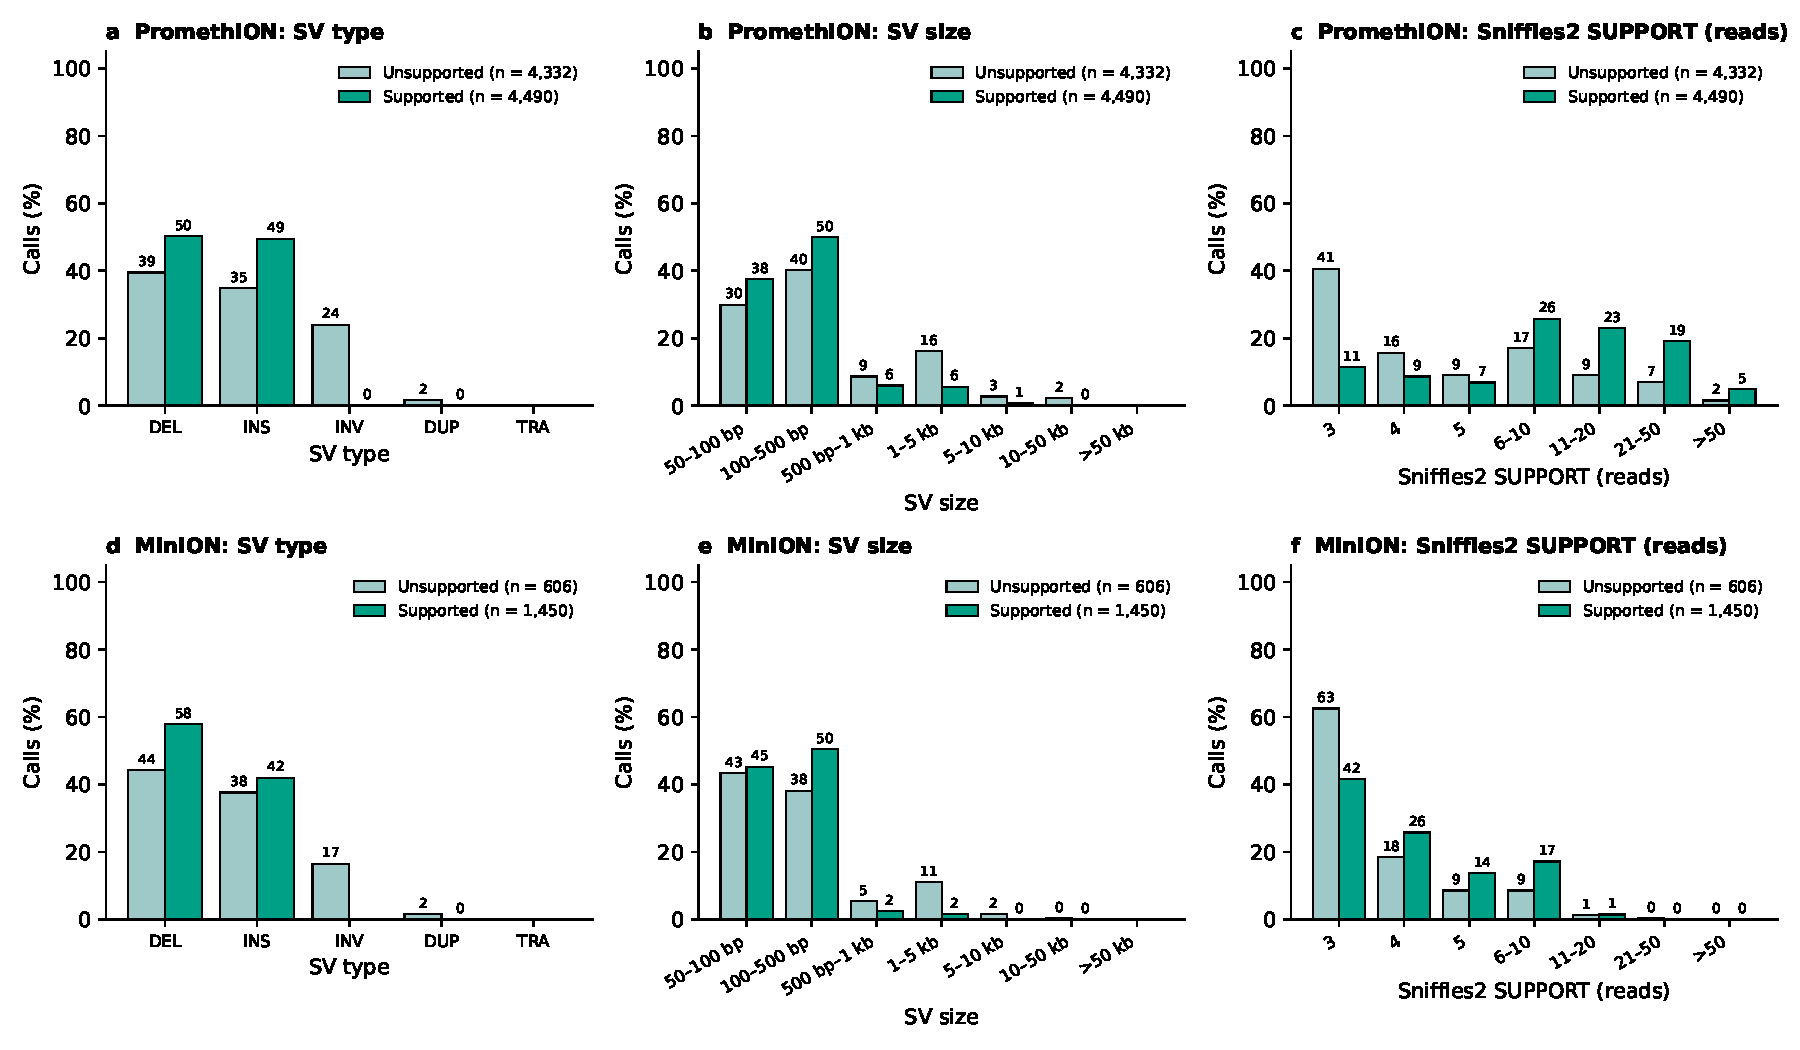
\includegraphics[width=\textwidth]{final_figures/sf_residual_sv}
	\end{center}
	\caption{{\bf Features of structural variant calls that remain unsupported after ChimeraLM filtering.}
		\gls{sv} calls from the \gls{wga} + ChimeraLM call sets ($\geq$3 supporting reads) benchmarked against the gold standard (Figure~3b,c of the main text) were split into unsupported (light teal; Truvari false positives) and supported (dark teal; Truvari true positives) calls.
		\textbf{(a--c)}~PromethION ($n = 4{,}332$ unsupported, $4{,}490$ supported): distribution of \gls{sv} type (a), \gls{sv} size (b) and Sniffles2 read support (c).
		\textbf{(d--f)}~The same for MinION ($n = 606$ unsupported, $1{,}450$ supported).
		Numbers above bars give the percentage of calls in each class.
	}\label{fig:residual_sv}
\end{figure}

\clearpage

\begin{figure}[!ht]
	\begin{center}
		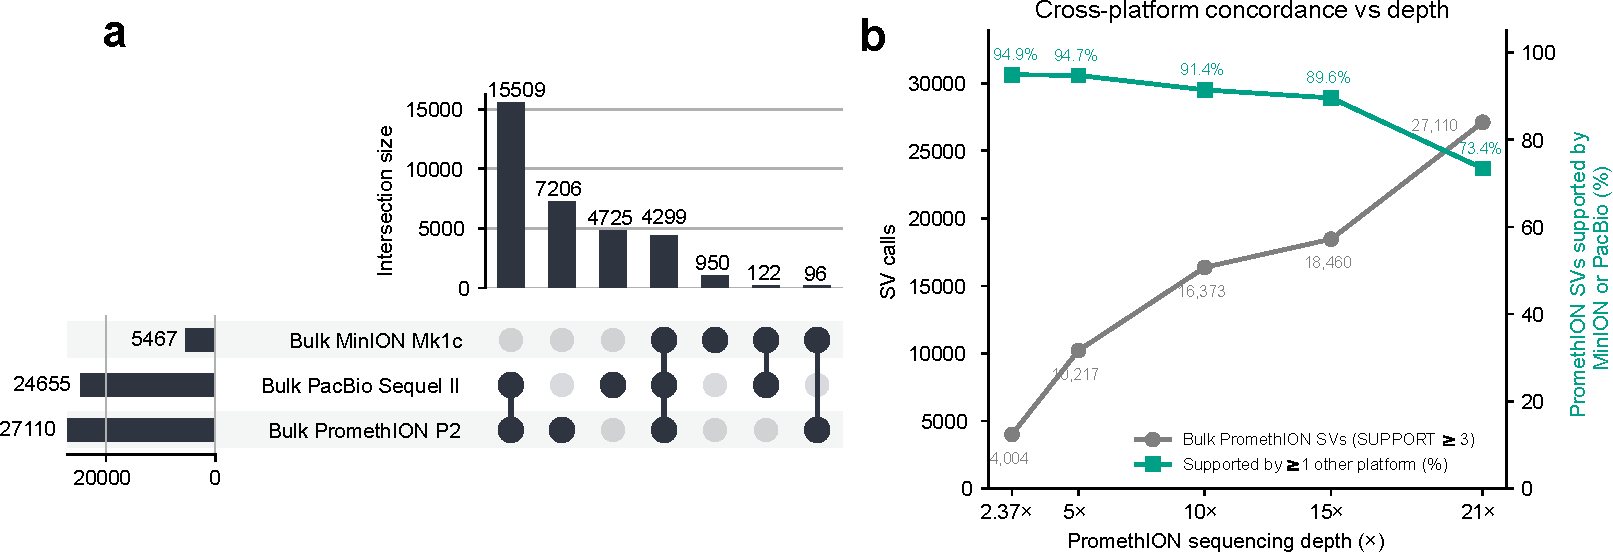
\includegraphics[width=\linewidth]{final_figures/sf_bulk_concordance}
	\end{center}
	\caption{{\bf Concordance of structural variant calls among the three bulk PC3 long-read datasets.}
		\textbf{(a)}~UpSet plot of high-confidence \glspl{sv} ($\geq$3 supporting reads; merged with OctopuSV) from bulk PromethION P2 (20.8$\times$; 27,110 calls), bulk MinION Mk1c (2.4$\times$; 5,467) and bulk PacBio Sequel~II (38$\times$; 24,655). Of the 32,907 union calls, 20,026 (60.9\%) are detected on at least two platforms and 4,299 (13.1\%) on all three; platform-private calls make up 26.6\%, 17.4\% and 19.2\% of the PromethION, MinION and PacBio call sets, respectively.
		\textbf{(b)}~Depth titration of the bulk PromethION data (down-sampled to 2.37$\times$, 5$\times$, 10$\times$, 15$\times$ and full 21$\times$): number of PromethION \gls{sv} calls (grey) and the fraction supported by at least one of the other two platforms (teal). The platform-private fraction rises with depth (5.1\% to 26.6\%), showing that deeper sequencing recovers variants absent from the shallower reference sets.
	}\label{fig:bulk_concordance}
\end{figure}

\clearpage

\begin{figure}[!ht]
	\begin{center}
		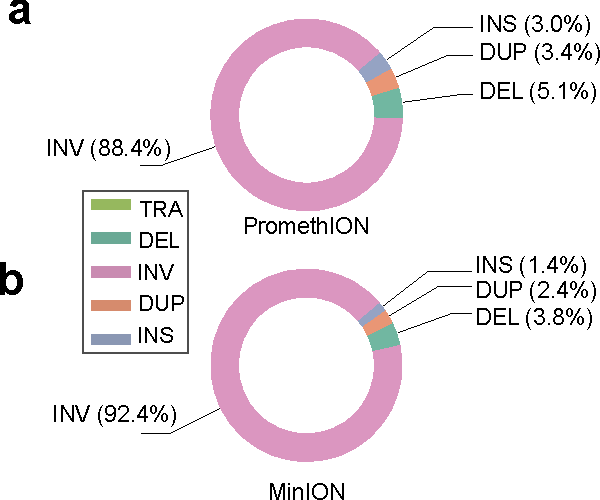
\includegraphics[width=0.9\textwidth]{final_figures/artifacts_suppoorted_sv}
	\end{center}
	\caption{{\bf Composition of artifact-supported \glspl{sv} for PromethION (a) and MinION (b).}
		Donut charts summarize the distribution of \gls{sv} types including \glsfirst{tra}, \glsfirst{del}, \glsfirst{inv}, \glsfirst{dup}, and \glsfirst{ins} among events supported exclusively by chimera artifacts, representing artificial \glspl{sv} preferentially removed by ChimeraLM (all Sniffles2 calls, without a minimum read-support filter).}\label{fig:sv_artifact_distribution}
\end{figure}

\clearpage

\glsaddall
\printglossary[type=\acronymtype,title={Abbreviations}]

\renewcommand{\bibname}{Supplementary References}
\renewcommand{\refname}{Supplementary References}
\bibliography{clean}

\end{document}
